\documentclass[letterpaper,11pt]{article}

\usepackage{latexsym}
\usepackage[empty]{fullpage}
\usepackage{titlesec}
\usepackage{marvosym}
\usepackage[usenames,dvipsnames]{color}
\usepackage{verbatim}
\usepackage{enumitem}
\usepackage[hidelinks]{hyperref}
\usepackage{fancyhdr}
\usepackage[english]{babel}
\usepackage{tabularx}
\usepackage{fontawesome5}
\usepackage{multicol}
\setlength{\multicolsep}{-3.0pt}
\setlength{\columnsep}{-1pt}
\input{glyphtounicode}

%new packages

\usepackage{fontenc}
\usepackage{amsmath}
\usepackage{amssymb}
\usepackage{graphicx}



%----------FONT OPTIONS----------

\pagestyle{fancy}
\fancyhf{} % clear all header and footer fields
\fancyfoot{}
\renewcommand{\headrulewidth}{0pt}
\renewcommand{\footrulewidth}{0pt}

% Adjust margins
\addtolength{\oddsidemargin}{-0.6in}
\addtolength{\evensidemargin}{-0.5in}
\addtolength{\textwidth}{1.19in}
\addtolength{\topmargin}{-.7in}
\addtolength{\textheight}{1.4in}

\urlstyle{same}

\raggedbottom
\raggedright
\setlength{\tabcolsep}{0in}

% Sections formatting
\titleformat{\section}{
  \vspace{-4pt}\scshape\raggedright\large\bfseries
}{}{0em}{}[\color{black}\titlerule \vspace{-5pt}]



% Ensure that generate pdf is machine readable/ATS parsable
\pdfgentounicode=1

%-------------------------
% Custom commands
\newcommand{\resumeItem}[1]{
  \item\small{
    {#1 \vspace{-2pt}}
  }
}

\newcommand{\classesList}[4]{
    \item\small{
        {#1 #2 #3 #4 \vspace{-2pt}}
  }
}

\newcommand{\resumeSubheading}[4]{
  \vspace{-2pt}\item
    \begin{tabular*}{1.0\textwidth}[t]{l@{\extracolsep{\fill}}r}
      \textbf{#1} & \textbf{\small #2} \\
      \textit{\small#3} & \textit{\small #4} \\
    \end{tabular*}\vspace{-7pt}
}

\newcommand{\resumeSubSubheading}[2]{
    \item
    \begin{tabular*}{0.97\textwidth}{l@{\extracolsep{\fill}}r}
      \textit{\small#1} & \textit{\small #2} \\
    \end{tabular*}\vspace{-7pt}
}

\newcommand{\resumeProjectHeading}[2]{
    \item
    \begin{tabular*}{1.001\textwidth}{l@{\extracolsep{\fill}}r}
      \small#1 & \textbf{\small #2}\\
    \end{tabular*}\vspace{-7pt}
}


\newcommand{\resumeSubItem}[1]{\resumeItem{#1}\vspace{-4pt}}

\renewcommand\labelitemi{$\vcenter{\hbox{\tiny$\bullet$}}$}
\renewcommand\labelitemii{$\vcenter{\hbox{\tiny$\bullet$}}$}

\newcommand{\resumeSubHeadingListStart}{\begin{itemize}[leftmargin=0.0in, label={}]}
\newcommand{\resumeSubHeadingListEnd}{\end{itemize}}
\newcommand{\resumeItemListStart}{\begin{itemize}}
\newcommand{\resumeItemListEnd}{\end{itemize}\vspace{-5pt}}


\begin{document}
\fontfamily{cmr}\selectfont
\begin{center}
\parbox{3.0cm}{%
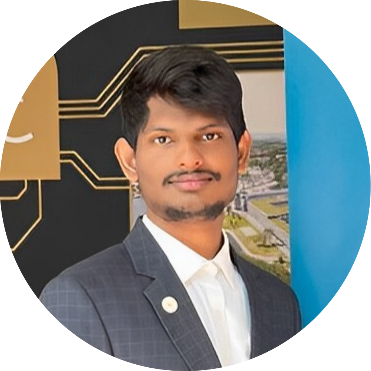
\includegraphics[width=2.7cm,clip]{images/resume_pic_m.png}}
\parbox{\dimexpr\linewidth-3.8cm\relax}{
\vspace{-20pt}
\begin{tabularx}{\linewidth}{L r} \\
    {\Huge \scshape  Venkata Sai Yakkshit Reddy Asodi}~
    \href{https://www.cedzlabs.com/yakkshit}{\vspace{1pt}}\\
      Berlin, Germany. \\ \vspace{1pt}
     \small \raisebox{-0.1\height}\faPhone\ +91 8179936156 ~ \href{mailto:saiyakkshit2001@gmail.com}{\raisebox{-0.2\height}\faEnvelope\  {saiyakkshit2001@gmail.com}} ~ 
    \href{https://linkedin.com/in/yakkshit/}{\raisebox{-0.2\height}\faLinkedin\ {yakkshit}}  ~
    \href{https://yakkshit.com/}{\raisebox{-0.2\height}\faGlobe\ {yakkshit.com}}  ~
    \href{https://github.com/yakkshit}{\raisebox{-0.2\height}\faGithub{ yakkshit}}
    \vspace{-8pt}
    
\end{tabularx}
}
\end{center}

\vspace{-23pt}
%-----------SUMMARY-----------
\section{Summary}
Highly motivated Full Stack Engineer with expertise in AI-driven solutions, frontend and backend development, and experience in leadership roles. Passionate about building scalable AI-powered products, with proven success in fast-paced startup environments. Skilled in optimizing LLMs and deploying low-code solutions for complex automation. Seeking a challenging role as a CTO to lead technical teams and drive innovation.

%-----------TECHNICAL SKILLS-----------
\section{Technical Skills}
\begin{itemize}[leftmargin=0.15in, label={}]
\small{\item{
\textbf{Languages: }{JavaScript (ES6+), Python, TypeScript, SQL.} \\
\textbf{Frameworks: }{React, Next.js, Django, Node.js, Retool.} \\
\textbf{AI/ML: }{LLMs, RAG, TensorFlow, OpenAI API.} \\
\textbf{Databases: }{PostgreSQL, MongoDB, Supabase.} \\
\textbf{Tools: }{Git, Docker, Kubernetes, AWS, Azure, Make.} \\
\textbf{Methodologies: }{Agile, Kanban, CI/CD.}
}}
\end{itemize}
\vspace{-10pt}

%-----------EXPERIENCE-----------
\section{Experience}

\resumeSubHeadingListStart

\resumeSubheading
{\large Circleup AG}{January 2024 -- July 2024}
  {Lead Full Stack Engineer (Frontend Focus)}{Zurich, Switzerland}\\
\vspace{10pt}
\textbf{Responsibilities:}
\resumeItemListStart
\vspace{-10pt}
\resumeItem{Developed AI-powered event scheduling and automation platforms, integrating OpenAI and ElevenLabs APIs for speech and text generation.}
\resumeItem{Led the architecture of scalable backend services using Django, optimized LLM models, and deployed applications on AWS.}
\resumeItem{Collaborated with cross-functional teams to define the product roadmap, ensuring a balance between innovation and operational efficiency.}
\resumeItemListEnd
\vspace{-3pt}
\textbf{Environment:}\emph{React, Django, OpenAI API, AWS, SQL, Agile.}

\resumeSubheading
{Cedzlabs}{March 2023 -- July 2024}
{Full Stack Developer}{Remote, India}\\
\vspace{10pt}
\textbf{Responsibilities:}
\vspace{-10pt}
\resumeItemListStart
\resumeItem{Built and maintained cloud-native applications with a focus on AI-driven solutions for SMBs, integrating low-code platforms like Retool and Airtable.}
\resumeItem{Enhanced product performance and user engagement through process automation, database optimization, and scalable API design.}
\resumeItemListEnd
\vspace{-3pt}
\textbf{Environment:}\emph{Next.js, Node.js, MongoDB, Azure.}

\resumeSubHeadingListEnd

%-----------PROJECTS-----------
\section{Projects}
\resumeSubHeadingListStart

\resumeProjectHeading
{\textbf{AI Resume Tuner} $|$ \emph{Azure Cloud, Next.js, LLMs}}{August 2024}\\
\vspace{6pt}
\textbf{Description:}
\vspace{-5pt}
\resumeItemListStart
\resumeItem{Developed an AI-powered resume tuning tool using RAG and LLMs, designed for users to input their career data and generate tailored resumes. Integrated backend APIs with a sleek Next.js frontend and deployed on Azure Cloud for scalability.}
\resumeItemListEnd
\vspace{4pt}
\textbf{Tools:}\emph{Azure Cloud, Next.js, OpenAI API, TailwindCSS.}

\resumeProjectHeading
{\textbf{Event Scheduling Platform} $|$ \emph{React, Django, OpenAI}}{January 2024}\\
\vspace{6pt}
\textbf{Description:}
\vspace{-5pt}
\resumeItemListStart
\resumeItem{Built a dynamic scheduling platform with real-time calendar integration using Google/Outlook APIs, voice automation via Twilio, and script generation using OpenAI.}
\resumeItemListEnd
\vspace{4pt}
\textbf{Tools:}\emph{React, Django, Twilio, OpenAI, Google API.}

\resumeSubHeadingListEnd

%-----------LANGUAGES-----------
\section{Languages}
\begin{itemize}
  \item English - Fluent $|$ German - Elementary $|$ Telugu - Native.
\end{itemize}

%-----------ACHIEVEMENTS-----------
\section{Achievements}
\begin{itemize}[leftmargin=0.15in, label={}]
\item Built and launched AI-powered products in two startups, increasing user engagement by 30\%. \\
\item Led recruitment and technical mentorship for engineering teams, growing team size by 50\%. \\
\item Contributed to open-source AI tools focused on automation.
\end{itemize}

\vspace{10pt}
\textbf{Strengths: }Leadership, adaptability, innovation, and strong technical skills.
\end{document}